% !TEX root = ../main.tex
\chapter{Dimensionality Reduction}
\label{ch:dimensionality}

\begin{intuition}[title=\textbf{The Blessing of Low-Dimensional Structure}]
Real-world data in $\R^p$ often lies near a much lower-dimensional manifold. Dimensionality reduction discovers this structure, enabling visualisation, noise removal, and faster downstream learning. We study linear methods (PCA) and nonlinear methods (kernel PCA, $t$-SNE, UMAP).
\end{intuition}

%% ----------------------------------------------------------------
\section{The Curse of Dimensionality}

\begin{proposition}[Volume of a Hypersphere]
The fraction of the volume of a $p$-dimensional unit hypercube $[0,1]^p$ captured by an inscribed hypersphere of radius $\tfrac{1}{2}$ is
\[
  \frac{V_p(\tfrac12)}{1} = \frac{\pi^{p/2}}{2^p\,\Gamma(\tfrac{p}{2}+1)}
  \xrightarrow{p\to\infty} 0.
\]
In high dimensions, almost all the volume concentrates in the corners.
\end{proposition}

\begin{proposition}[Concentration of Distances]
For $n$ points drawn uniformly in $[0,1]^p$, the ratio of the maximum to minimum pairwise distances converges to 1:
\[
  \frac{d_{\max} - d_{\min}}{d_{\min}} \xrightarrow{p\to\infty} 0 \quad\text{in probability}.
\]
Distance-based methods (e.g.\ $k$-NN, $k$-means) lose discriminative power.
\end{proposition}

\begin{warning}[title=\textbf{Practical Consequences}]
\begin{itemize}
  \item Sample complexity grows exponentially with $p$ for non-parametric methods.
  \item Nearest-neighbour distances become nearly indistinguishable.
  \item Overfitting risk increases: many spurious correlations in high dimensions.
\end{itemize}
\end{warning}

%% ----------------------------------------------------------------
\section{Principal Component Analysis (PCA)}

\subsection{Derivation via Variance Maximisation}

\begin{definition}[PCA]
Let $\bm{X}\in\R^{n\times p}$ be the centred data matrix ($\bar{\bm{x}}=\bm{0}$). PCA seeks the orthogonal directions of maximum variance. The first principal component direction is
\[
  \bm{w}_1 = \argmax_{\norm{\bm{w}}=1} \Var[\bm{X}\bm{w}]
  = \argmax_{\norm{\bm{w}}=1} \bm{w}^\top\bm{S}\bm{w},
\]
where $\bm{S}=\frac{1}{n-1}\bm{X}^\top\bm{X}$ is the sample covariance matrix.
\end{definition}

\begin{theorem}[PCA via Eigendecomposition]
The solution to the PCA problem is given by the eigenvectors of $\bm{S}$. If $\bm{S}=\bm{W}\bm{\Lambda}\bm{W}^\top$ with eigenvalues $\lambda_1\geq\lambda_2\geq\cdots\geq\lambda_p\geq 0$, then:
\begin{enumerate}
  \item The $k$-th principal component direction is $\bm{w}_k$ (the $k$-th eigenvector).
  \item The variance captured by $\bm{w}_k$ is $\lambda_k$.
  \item The proportion of total variance explained by the first $d$ components is $\sum_{k=1}^d\lambda_k / \sum_{k=1}^p\lambda_k$.
\end{enumerate}
\end{theorem}

\begin{proof}
By the method of Lagrange multipliers with constraint $\norm{\bm{w}}=1$:
\[
  \nabla_{\bm{w}}\bigl[\bm{w}^\top\bm{S}\bm{w} - \lambda(\bm{w}^\top\bm{w}-1)\bigr] = \bm{0}
  \quad\Longrightarrow\quad \bm{S}\bm{w} = \lambda\bm{w}.
\]
So $\bm{w}$ must be an eigenvector of $\bm{S}$, and the objective value is $\bm{w}^\top\bm{S}\bm{w}=\lambda$. The maximum is achieved at the eigenvector with the largest eigenvalue. The subsequent components are obtained by restricting to the orthogonal complement of the previously selected directions; by the spectral theorem, these are precisely the remaining eigenvectors in decreasing eigenvalue order.
\end{proof}

\subsection{PCA via Singular Value Decomposition}

\begin{theorem}[SVD Formulation of PCA]
Let $\bm{X}=\bm{U}\bm{D}\bm{V}^\top$ be the (thin) SVD, where $\bm{U}\in\R^{n\times p}$, $\bm{D}=\operatorname{diag}(\sigma_1,\dots,\sigma_p)$, $\bm{V}\in\R^{p\times p}$ orthogonal. Then:
\begin{enumerate}
  \item The principal component directions are the columns of $\bm{V}$.
  \item The eigenvalues of $\bm{S}$ are $\lambda_k = \sigma_k^2/(n-1)$.
  \item The principal component scores are $\bm{Z}=\bm{X}\bm{V}=\bm{U}\bm{D}$.
\end{enumerate}
The SVD is numerically more stable than explicitly forming $\bm{S}=\bm{X}^\top\bm{X}/(n-1)$.
\end{theorem}

\begin{proposition}[PCA as Optimal Low-Rank Approximation]
The rank-$d$ truncation $\bm{X}_d=\bm{U}_d\bm{D}_d\bm{V}_d^\top$ (retaining the top $d$ singular values) solves
\[
  \min_{\operatorname{rank}(\bm{M})\leq d}\norm{\bm{X}-\bm{M}}_F^2,
\]
by the Eckart--Young--Mirsky theorem. The reconstruction error is $\sum_{k=d+1}^p\sigma_k^2$.
\end{proposition}

\subsection{Scree Plots and Choosing $d$}

\begin{bestpractice}[title=\textbf{Selecting the Number of Components}]
\begin{itemize}
  \item \textbf{Scree plot}: plot $\lambda_k$ vs $k$; look for an ``elbow''.
  \item \textbf{Cumulative variance}: choose $d$ such that $\sum_{k=1}^d\lambda_k/\sum_{k=1}^p\lambda_k\geq\tau$ (e.g.\ $\tau=0.95$).
  \item \textbf{Kaiser's rule}: retain components with $\lambda_k>1$ (on standardised data).
\end{itemize}
\end{bestpractice}

\begin{figure}[ht]
\centering
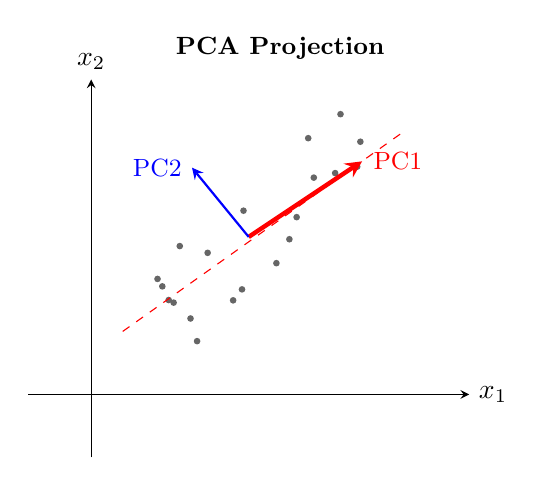
\begin{tikzpicture}[scale=0.8]
  \begin{scope}
    \node[font=\bfseries\small] at (3,5.5) {PCA Projection};
    \draw[-stealth] (-1,0) -- (6,0) node[right]{$x_1$};
    \draw[-stealth] (0,-1) -- (0,5) node[above]{$x_2$};
    % Data cloud
    \foreach \i in {1,...,20}{
      \pgfmathsetmacro{\ax}{2.5+1.8*rand}
      \pgfmathsetmacro{\ay}{2.5+1.2*rand+0.6*\ax-1.5}
      \fill[black!60] (\ax,\ay) circle(1.5pt);
    }
    % PC1 direction
    \draw[red, ultra thick, -stealth] (2.5,2.5) -- (4.3,3.7)
      node[right,font=\small]{PC1};
    % PC2 direction
    \draw[blue, thick, -stealth] (2.5,2.5) -- (1.6,3.6)
      node[left,font=\small]{PC2};
    % Projection line
    \draw[red, dashed] (0.5,1.0) -- (5.0,4.2);
  \end{scope}
\end{tikzpicture}
\caption{PCA finds the directions of maximum variance. The first principal component (red) captures the most variance; the second (blue) is orthogonal to it.}
\label{fig:pca-projection}
\end{figure}

%% ----------------------------------------------------------------
\section{Kernel PCA}

\begin{definition}[Kernel PCA]
Kernel PCA performs PCA in a feature space $\mathcal{H}$ induced by a kernel $\kappa$. Given the kernel matrix $\bm{K}\in\R^{n\times n}$ with $K_{ij}=\kappa(\bm{x}_i,\bm{x}_j)$, the centred kernel matrix is
\[
  \tilde{\bm{K}} = \bm{K} - \bm{1}_n\bm{K} - \bm{K}\bm{1}_n + \bm{1}_n\bm{K}\bm{1}_n,
\]
where $\bm{1}_n = \frac{1}{n}\bm{11}^\top$. The principal components in feature space are obtained from the eigendecomposition $\tilde{\bm{K}}=\bm{U}\bm{\Lambda}\bm{U}^\top$, and the projections are $\bm{Z}=\bm{U}\bm{\Lambda}^{1/2}$.
\end{definition}

%% ----------------------------------------------------------------
\section{$t$-SNE}

\begin{definition}[$t$-SNE]
$t$-distributed Stochastic Neighbour Embedding ($t$-SNE) maps high-dimensional data to a low-dimensional space (typically $d=2$) by matching pairwise similarity distributions.

In high-dimensional space, define symmetric similarities:
\[
  p_{ij} = \frac{p_{j|i} + p_{i|j}}{2n}, \qquad
  p_{j|i} = \frac{\exp(-\norm{\bm{x}_i-\bm{x}_j}^2 / 2\sigma_i^2)}{\sum_{k\neq i}\exp(-\norm{\bm{x}_i-\bm{x}_k}^2 / 2\sigma_i^2)}.
\]
In low-dimensional space, use a Student $t$-distribution with one degree of freedom:
\[
  q_{ij} = \frac{(1+\norm{\bm{y}_i-\bm{y}_j}^2)^{-1}}{\sum_{k\neq \ell}(1+\norm{\bm{y}_k-\bm{y}_\ell}^2)^{-1}}.
\]
The embedding $\{\bm{y}_i\}$ is found by minimising the KL divergence:
\[
  \mathcal{L} = \KL(P\|Q) = \sum_{i\neq j} p_{ij}\ln\frac{p_{ij}}{q_{ij}}.
\]
\end{definition}

\begin{remark}
The bandwidth $\sigma_i$ for each point is set so that the conditional distribution $p_{\cdot|i}$ has a specified \emph{perplexity}, defined as $\text{Perp}(P_i)=2^{H(P_i)}$ where $H$ is the Shannon entropy. Typical values are 5--50.
\end{remark}

\begin{warning}[title=\textbf{$t$-SNE Caveats}]
\begin{itemize}
  \item Cluster sizes and inter-cluster distances in the plot are \emph{not} meaningful.
  \item Results depend on perplexity and random initialisation; always try several settings.
  \item $t$-SNE is primarily a \emph{visualisation} tool; do not use the embeddings for downstream tasks.
\end{itemize}
\end{warning}

%% ----------------------------------------------------------------
\section{UMAP}

\begin{definition}[UMAP]
Uniform Manifold Approximation and Projection (UMAP) models the data as lying on a Riemannian manifold. It constructs a weighted $k$-nearest-neighbour graph in high dimensions and optimises a low-dimensional layout to match the topological structure via cross-entropy minimisation:
\[
  \mathcal{L}_{\text{UMAP}} = \sum_{(i,j)} \bigl[w_{ij}\ln\frac{w_{ij}}{v_{ij}} + (1-w_{ij})\ln\frac{1-w_{ij}}{1-v_{ij}}\bigr],
\]
where $w_{ij}$ and $v_{ij}$ are edge weights in the high- and low-dimensional graphs respectively.
\end{definition}

\begin{bestpractice}[title=\textbf{$t$-SNE vs UMAP}]
\begin{itemize}
  \item UMAP is generally faster (approximate nearest-neighbour search).
  \item UMAP better preserves global structure.
  \item UMAP embeddings can be used for downstream tasks (unlike $t$-SNE).
  \item Key UMAP hyperparameters: \texttt{n\_neighbors} (local vs global), \texttt{min\_dist} (tightness).
\end{itemize}
\end{bestpractice}

%% ----------------------------------------------------------------
\section{Implementation in Python}

\begin{codeblock}[title=\textbf{PCA from Scratch}]
\begin{minted}{python}
import numpy as np

def pca_from_scratch(X, n_components):
    """PCA via eigendecomposition of the covariance matrix."""
    # Centre the data
    X_centered = X - X.mean(axis=0)
    # Covariance matrix
    n = X_centered.shape[0]
    S = X_centered.T @ X_centered / (n - 1)
    # Eigendecomposition
    eigenvalues, eigenvectors = np.linalg.eigh(S)
    # Sort in descending order
    idx = np.argsort(eigenvalues)[::-1]
    eigenvalues = eigenvalues[idx]
    eigenvectors = eigenvectors[:, idx]
    # Project
    W = eigenvectors[:, :n_components]
    Z = X_centered @ W
    explained_var_ratio = eigenvalues[:n_components] / eigenvalues.sum()
    return Z, eigenvalues, explained_var_ratio

# Test on Iris
from sklearn.datasets import load_iris
X_iris = load_iris().data
Z, eigenvals, ratios = pca_from_scratch(X_iris, 2)
print(f"Explained variance ratios: {ratios}")
print(f"Total: {ratios.sum():.4f}")
\end{minted}
\end{codeblock}

\begin{codeoutput}
\begin{verbatim}
Explained variance ratios: [0.92461872 0.05306648]
Total: 0.9777
\end{verbatim}
\end{codeoutput}

\begin{codeblock}[title=\textbf{PCA, Kernel PCA, $t$-SNE, and UMAP with scikit-learn}]
\begin{minted}{python}
import numpy as np
import matplotlib.pyplot as plt
from sklearn.datasets import load_digits
from sklearn.preprocessing import StandardScaler
from sklearn.decomposition import PCA, KernelPCA
from sklearn.manifold import TSNE

X, y = load_digits(return_X_y=True)
X = StandardScaler().fit_transform(X)

# PCA
pca = PCA(n_components=2)
X_pca = pca.fit_transform(X)
print(f"PCA explained variance: {pca.explained_variance_ratio_.sum():.3f}")

# Scree plot
pca_full = PCA().fit(X)
fig, (ax1, ax2) = plt.subplots(1, 2, figsize=(10, 4))
ax1.plot(np.cumsum(pca_full.explained_variance_ratio_), "b-o", markersize=3)
ax1.axhline(0.95, color="r", linestyle="--", label="95% threshold")
ax1.set_xlabel("Number of components"); ax1.set_ylabel("Cumulative variance")
ax1.set_title("Scree Plot"); ax1.legend()

# Kernel PCA (RBF)
kpca = KernelPCA(n_components=2, kernel="rbf", gamma=0.01)
X_kpca = kpca.fit_transform(X)

# t-SNE
tsne = TSNE(n_components=2, perplexity=30, random_state=42)
X_tsne = tsne.fit_transform(X)

# Plot all
methods = {"PCA": X_pca, "Kernel PCA": X_kpca, "t-SNE": X_tsne}
fig, axes = plt.subplots(1, 3, figsize=(15, 4))
for ax, (name, Z) in zip(axes, methods.items()):
    scatter = ax.scatter(Z[:, 0], Z[:, 1], c=y, cmap="tab10", s=5, alpha=0.7)
    ax.set_title(name); ax.set_xticks([]); ax.set_yticks([])
plt.tight_layout()
plt.savefig("figures/ch09_dim_reduction.pdf")
\end{minted}
\end{codeblock}

\begin{codeblock}[title=\textbf{UMAP (requires \texttt{umap-learn} package)}]
\begin{minted}{python}
import umap

reducer = umap.UMAP(n_components=2, n_neighbors=15, min_dist=0.1,
                     random_state=42)
X_umap = reducer.fit_transform(X)

fig, (ax1, ax2) = plt.subplots(1, 2, figsize=(10, 4))
ax1.scatter(X_tsne[:, 0], X_tsne[:, 1], c=y, cmap="tab10", s=5)
ax1.set_title("t-SNE")
ax2.scatter(X_umap[:, 0], X_umap[:, 1], c=y, cmap="tab10", s=5)
ax2.set_title("UMAP")
plt.tight_layout()
plt.savefig("figures/ch09_tsne_vs_umap.pdf")
\end{minted}
\end{codeblock}

%% ----------------------------------------------------------------
\section{Exercises}

\begin{exercise}[PCA Eigendecomposition]
Let $\bm{X}\in\R^{n\times 2}$ with sample covariance $\bm{S}=\begin{pmatrix}4 & 2\\2 & 3\end{pmatrix}$. Compute the eigenvalues and eigenvectors of $\bm{S}$. What proportion of variance is explained by the first principal component?
\end{exercise}

\begin{exercise}[SVD and PCA]
Show that for centred data $\bm{X}=\bm{U}\bm{D}\bm{V}^\top$, the eigenvalues of $\bm{S}=\bm{X}^\top\bm{X}/(n-1)$ are $\sigma_k^2/(n-1)$, where $\sigma_k$ are the singular values. Verify this numerically on the Iris dataset.
\end{exercise}

\begin{exercise}[Reconstruction Error]
Implement PCA on the digits dataset ($p=64$). Plot the reconstruction error $\norm{\bm{X}-\bm{X}_d}_F^2/\norm{\bm{X}}_F^2$ as a function of $d$ for $d=1,\dots,64$. At what $d$ does the error drop below 5\%?
\end{exercise}

\begin{exercise}[$t$-SNE Perplexity]
Run $t$-SNE on the digits dataset with perplexity values in $\{5, 15, 30, 50, 100\}$. For each, visualise the 2D embedding coloured by digit label. How does perplexity affect cluster separation and overall layout?
\end{exercise}

\begin{exercise}[Kernel PCA for Non-Linear Data]
Generate concentric circles using \texttt{make\_circles(n\_samples=500, factor=0.3, noise=0.05)}. Show that standard PCA fails to separate the two circles, but kernel PCA with an RBF kernel succeeds. Experiment with the $\gamma$ parameter.
\end{exercise}
